\documentclass[8pt]{beamer}
\usepackage{tikz}
\usepackage[utf8]{vietnam}
\usepackage{amsmath}
\usepackage{graphicx}
\usepackage{wrapfig}
\usepackage{hyperref}
\usepackage{mathrsfs}
\usetheme{Copenhagen}
\usecolortheme{dolphin}
\setbeamertemplate{navigation symbols}{}
\setbeamertemplate{headline}{}
\title[Chương 2: Cấu trúc hệ thống] %optional
{Chương 2: Cấu trúc hệ thống}
\subtitle{Xử lý tín hiệu số}
\author[Xử lý tín hiệu số] % (optional)
{Tín Vũ}
\date[VLC 2021] % (optional)
{tinvu1309@gmail.com}
\begin{document}
\frame{\titlepage}
\begin{frame}{Mục lục}
\tableofcontents
\end{frame}
\begin{frame}{Giới thiệu playlist}
\section{Giới thiệu playlist}
	\begin{itemize}
		\item Mình là Tín Vũ, hiện đang là sinh viên học tại Trường Đại học Công nghệ, Đại học Quốc gia Hà Nội. Mình tạo playlist video này để hỗ trợ các bạn học môn \textbf{Xử lý tín hiệu số}.
\item Khác với môn học tiên quyết \alert{Tín hiệu hệ thống} trước đó, bài giảng môn học này \textbf{hoàn toàn bám sát với đề cương và giáo trình nội bộ} của trường mình, nên các bạn trường khác cần phải lưu ý rất kĩ điều này.
\item Không chỉ dừng lại ở lý thuyết, playlist này \textbf{có bổ sung hướng dẫn lập trình cơ bản bằng GNU Octave/Matlab} để vẽ phổ tín hiệu, đáp ứng tần số và thiết kế bộ lọc.
\item Môn học này bao gồm \textbf{6 chương}, các chương đều liên quan rất chặt chẽ với nhau nên hãy học cẩn thận ngay từ \alert{Chương 0} để ôn thi cuối kì đỡ vất vả.
	\end{itemize}
\end{frame}
\begin{frame}{Tài liệu tham khảo}
\section{Tài liệu tham khảo}
\begin{itemize}
		\item Tài liệu tham khảo chính: Giáo trình Xử lý tín hiệu số (Nguyễn Linh Trung, Trần Đức Tân, Huỳnh Hữu Tuệ, ĐHCN, 2012).
		\item Tài liệu tham khảo phụ: Discrete-time Signal Processing (Alan V.Oppenheim, 2nd edition). 
	\end{itemize}
\end{frame}
\begin{frame}{Quy trình xử lý tín hiệu số}
\section{Quy trình xử lý tín hiệu số}
\begin{figure}[h]
			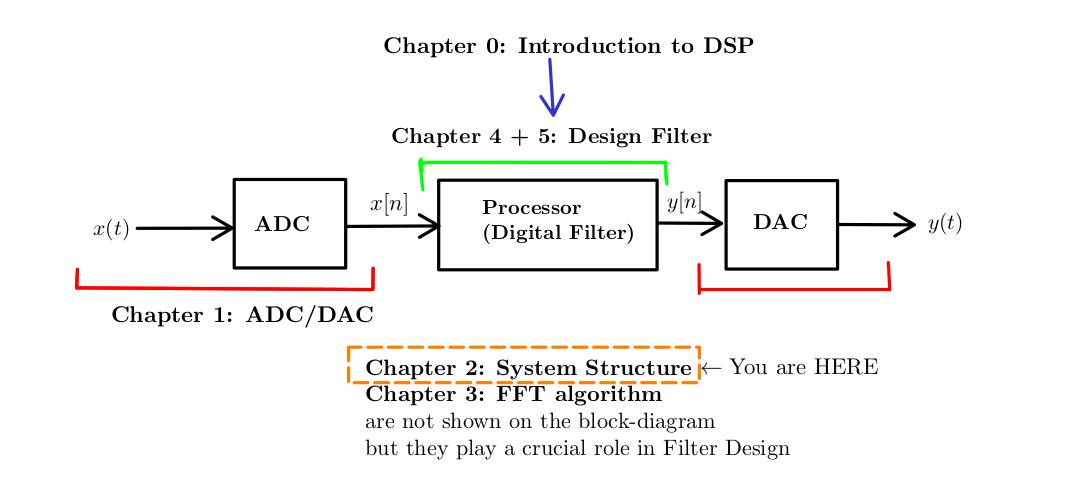
\includegraphics[width=1.1\textwidth]{1.jpg}
			\caption{DSP Learning Process}			\label{fig:re1}
		\end{figure}

\end{frame}
\begin{frame}{Các phần tử hạt nhân cấu thành hệ thống rời rạc}
\section{Các phần tử hạt nhân cấu thành hệ thống rời rạc}
\begin{figure}[h]
			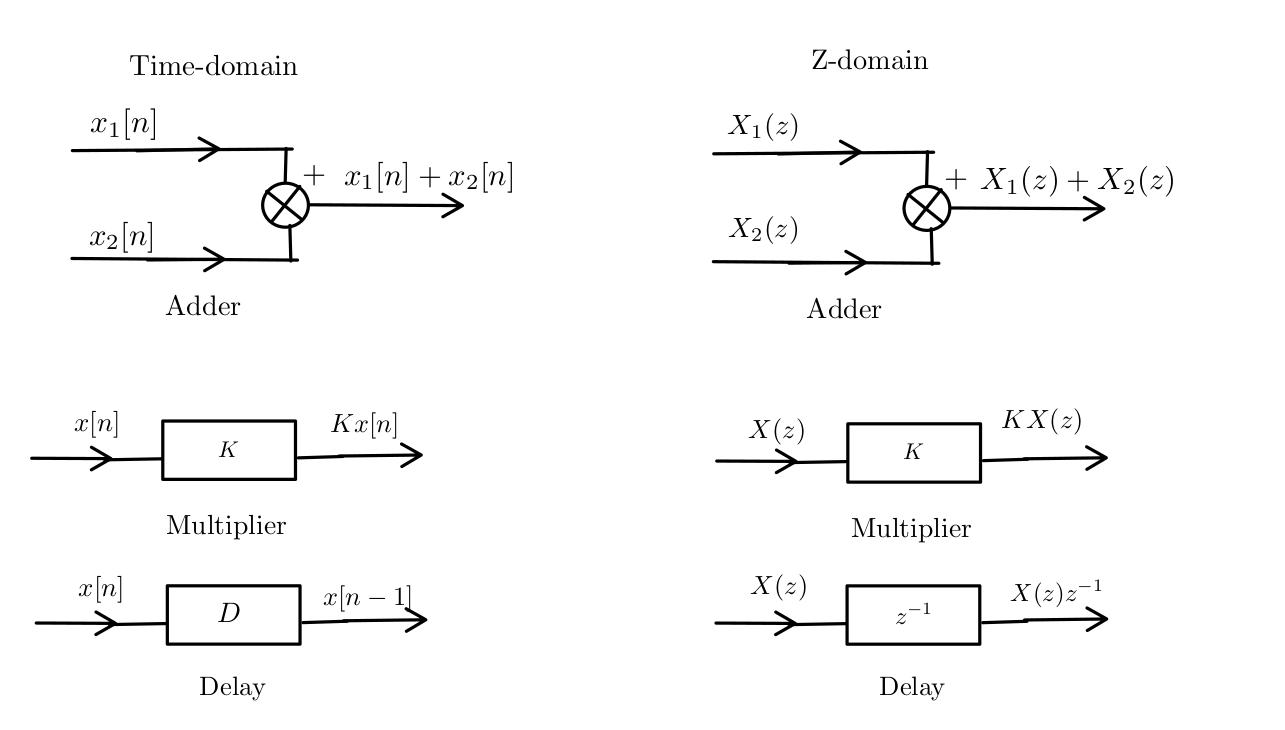
\includegraphics[width=1.1\textwidth]{2.jpg}
			\caption{Elementary components of system structure}			\label{fig:re2}
		\end{figure}
\end{frame}
\begin{frame}{Các phần tử hạt nhân cấu thành hệ thống rời rạc}
\begin{figure}[h]
			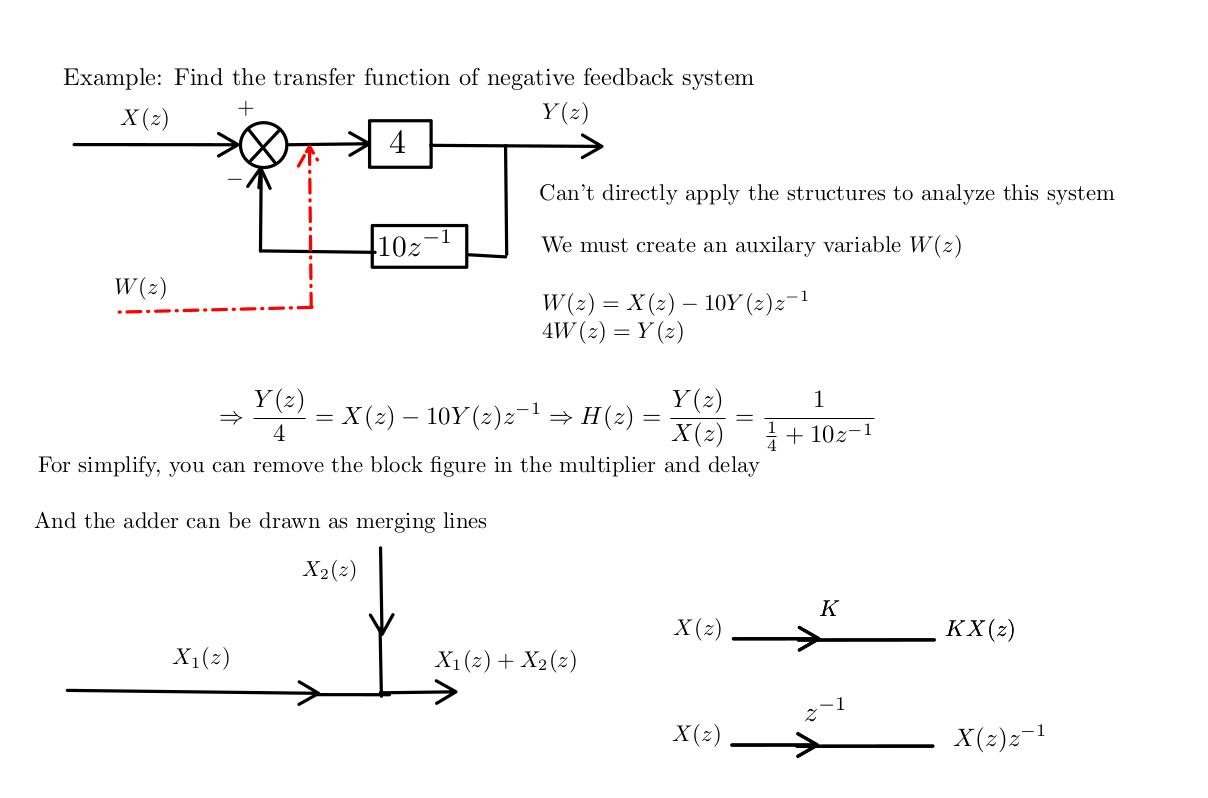
\includegraphics[width=1\textwidth]{3.jpg}
			\caption{Introduction to Signal-Flow graph}			\label{fig:re3}

		\end{figure}
\end{frame}
\begin{frame}{Cấu trúc hệ thống}
\begin{itemize}
	\item Cấu trúc hệ thống loại I
\end{itemize}
\section{Cấu trúc hệ thống}
\subsection{Cấu trúc hệ thống loại I}
Ta xét phương trình sai phân tổng quát biểu diễn hệ thống rời rạc:
\begin{equation*}
	\begin{split}
		\sum_{k=0}^{N}a_{k}y[n-k]&=\sum_{k=0}^{M}b_{k}x[n-k]\\
		\Rightarrow \mathscr{Z}\left(\sum_{k=0}^{N}a_{k}y[n-k]\right)&=\mathscr{Z}\left(\sum_{k=0}^{M}b_{k}x[n-k]\right)\\
		\Rightarrow Y(z)\left(\sum_{k=0}^{N}a_{k}z^{-k}\right)&=X(z)\left(\sum_{k=0}^{M}b_{k}z^{-k}\right)
	\end{split}
\end{equation*}
Nếu ta chia cả $2$ về cho hệ số $a_{0}$ và bỏ qua độ lớn thực của các hệ số sau khi chia (tức là ta không quan tâm đến giá trị của hệ số mà chỉ quan tâm đến tỷ lệ giữa chúng với nhau):
\begin{equation*}
\begin{split}
	Y(z)+Y(z)\sum_{k=1}^{N}a_{k}z^{-k}&=X(z)\left(\sum_{k=0}^{M}b_{k}z^{-k}\right)\\
	\Rightarrow Y(z)&=X(z)\left(\sum_{k=0}^{M}b_{k}z^{-k}\right)-Y(z)\sum_{k=1}^{N}a_{k}z^{-k}
\end{split}
\end{equation*}
Biểu diễn kết quả trên dưới dạng sơ đồ khối hoặc lưu đồ tín hiệu (từ giờ ta sẽ chỉ biểu diễn bằng lưu đồ tín hiệu), ta thu được cấu trúc hệ thống loại I.
\end{frame}
\begin{frame}{Cấu trúc hệ thống}
\begin{figure}[h]
			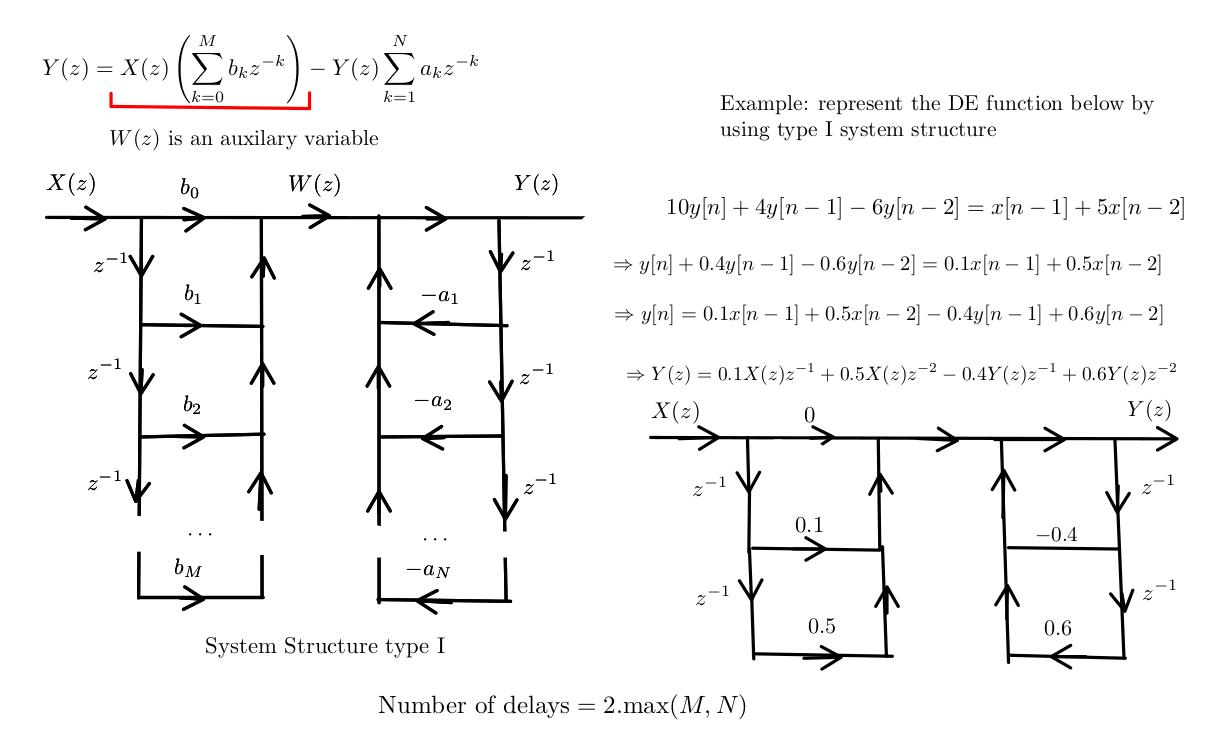
\includegraphics[width=1.1\textwidth]{4.jpg}
			\caption{System structure type I}			\label{fig:re4}

		\end{figure}

\end{frame}
\begin{frame}{Cấu trúc hệ thống}
\subsection{Cấu trúc hệ thống loại II}
\begin{itemize}
	\item Cấu trúc hệ thống loại II
\end{itemize}
Từ phương trình DE biểu diễn hệ thống rời rạc tổng quát, ta sẽ viết lại dưới dạng hàm truyền để xây dựng cấu trúc tối ưu mới:
\begin{equation*}
\begin{split}
	H(z)=\frac{Y(z)}{X(z)}=\frac{\sum_{k=0}^{M}b_{k}z^{-k}}{1+\sum_{k=1}^{N}a_{k}z^{-k}}&=\left(\sum_{k=0}^{M}b_{k}z^{-k}\right)\left(\frac{1}{1+\sum_{k=1}^{N}a_{k}z^{-k}}\right)\\
											    &=\alert{\left(\frac{1}{1+\sum_{k=1}^{N}a_{k}z^{-k}}\right)\left(\sum_{k=0}^{M}b_{k}z^{-k}\right)}\\
											    \end{split}
\end{equation*}
\begin{equation*}
\begin{split}
	\Rightarrow Y(z)&=\left(X(z)\sum_{k=0}^{M}b_{k}z^{-k}\right)\left(\frac{1}{1+\sum_{k=1}^{N}a_{k}z^{-k}}\right)=W(z)\left(\frac{1}{1+\sum_{k=1}^{N}a_{k}z^{-k}}\right)\textbf{ (Type I) }\\
			&=\left(\frac{X(z)}{1+\sum_{k=1}^{N}a_{k}z^{-k}}\right)\left(\sum_{k=0}^{M}b_{k}z^{-k}\right)=W(z)\left(\sum_{k=0}^{M}b_{k}z^{-k}\right)\textbf{ (Type II) }
\end{split}
\end{equation*}
Từ phương trình biến phụ $W(z)$, ta biến đổi được:
\begin{equation*}
\begin{split}
	X(z)&=W(z)+W(z)\sum_{k=1}^{N}a_{k}z^{-k}\\
	\Rightarrow W(z)&=X(z)-\sum_{k=1}^{N}a_{k}z^{-k}W(z)\\
\end{split}
\end{equation*}
\end{frame}
\begin{frame}{Cấu trúc hệ thống}
\begin{figure}[h]
			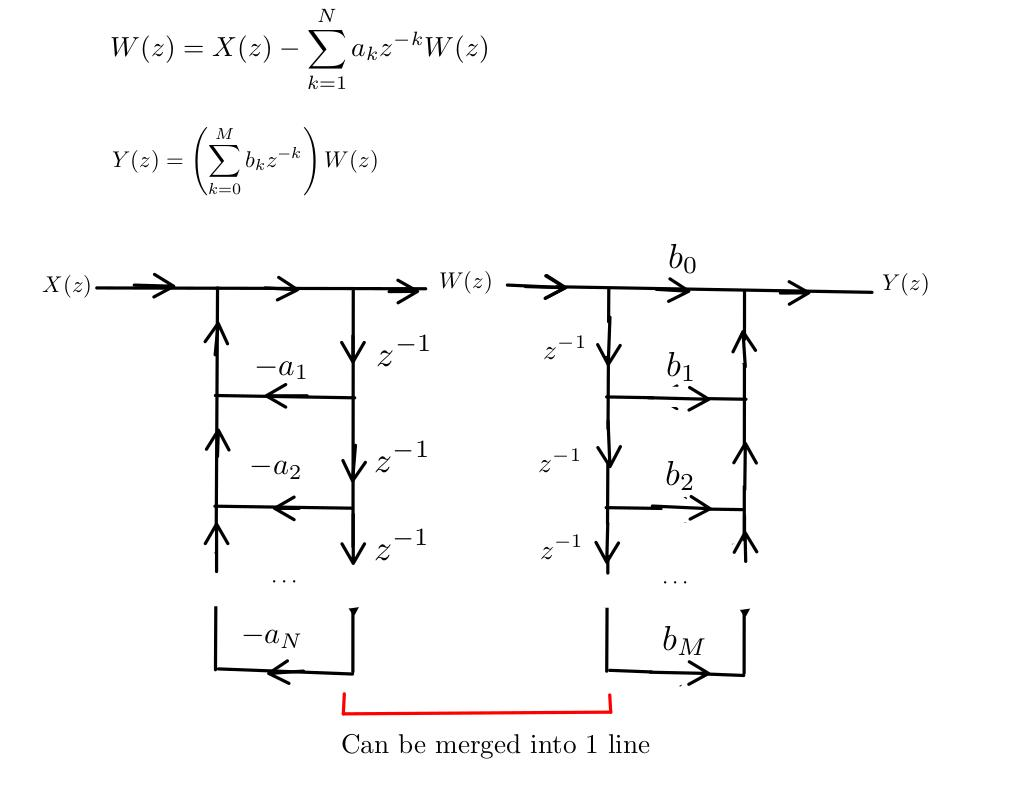
\includegraphics[width=0.8\textwidth]{5.jpg}
			\caption{System structure type II}			\label{fig:re5}

		\end{figure}
\end{frame}
\begin{frame}{Cấu trúc hệ thống}
\begin{figure}[h]
			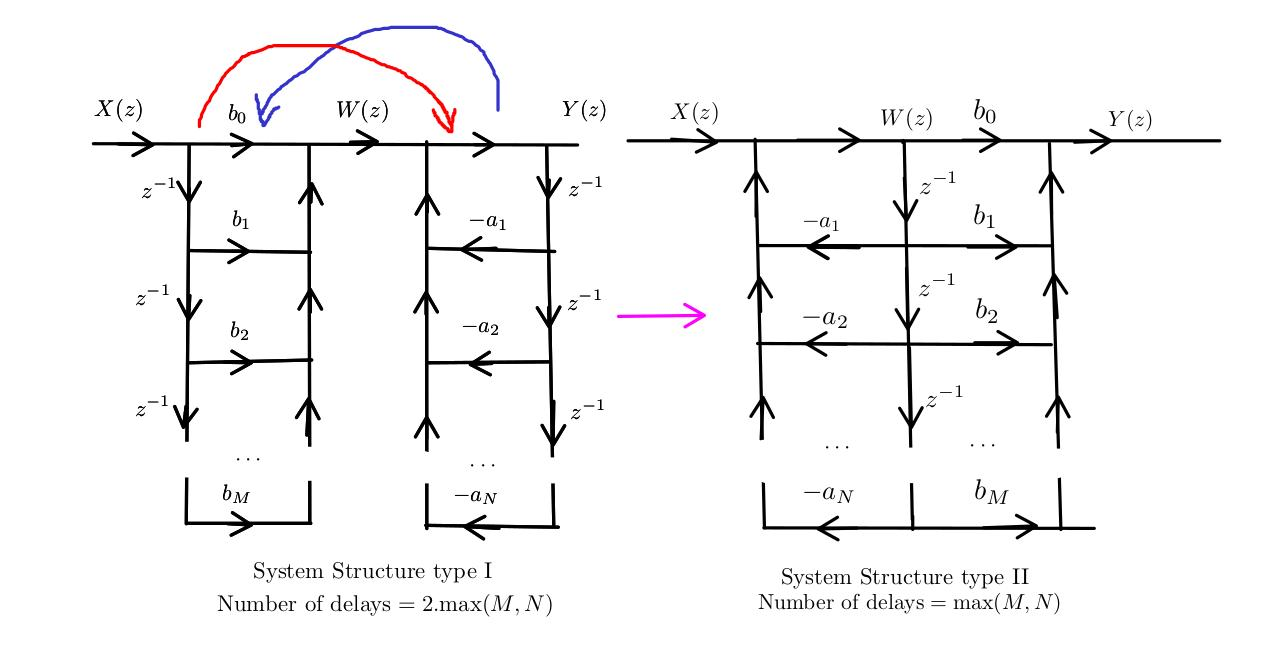
\includegraphics[width=0.7\textwidth]{6.jpg}
			\caption{System structure type I and II comparison}			\label{fig:re6}

		\end{figure}
	Đối với hệ thống bậc cao, thường ta sẽ tách hàm truyền ra thành \textbf{dạng tổng} (cấu trúc song song) hoặc \textbf{dạng tích} (cấu trúc nối tiếp) để đảm bảo hệ thống thiết kế tối ưu về hiệu suất, tính ổn định và chi phí sản xuất.

	$$H(z)=\sum_{k=0}^{N-1}H_{k}(z)\text{ (Parallel form) }$$
	$$H(z)=\prod_{k=0}^{N-1}H_{k}(z)\text{ (Cascade form) }$$
\end{frame}
\begin{frame}{Phân loại hệ thống}
\section{Phân loại hệ thống}
Từ hàm truyền tổng quát của hệ thống rời rạc:
$$H(z)=\frac{\sum_{k=0}^{M}b_{k}z^{-k}}{1+\sum_{k=1}^{N}a_{k}z^{-k}}$$
Nếu $a_{k}=0\; (\forall k)$, ta viết lại hàm truyền: $$H(z)=\frac{Y(z)}{X(z)}=\sum_{k=0}^{M}b_{k}z^{-k}\Rightarrow Y(z)=X(z)\sum_{k=0}^{M}b_{k}z^{-k}$$
Lấy biến đổi Z ngược 2 vế, ta có:
$$y[n]=\sum_{k=0}^{M}b_{k}x[n-k]$$
Ta thấy tín hiệu đầu ra $y[n]$ chỉ được cấu thành bởi tổng \alert{hữu hạn} tuyến tính các dịch trễ của tín hiệu đầu vào $x[n]$. Tiếp tục lấy biến đổi Z ngược để tìm đáp ứng xung của hệ thống:
$$\mathscr{Z}^{-1}(H(z))=\mathscr{Z}^{-1}\left(\sum_{k=0}^{M}b_{k}z^{-k}\right)\Rightarrow h[n]=\sum_{k=0}^{M}b_{k}\delta[n-k]$$
Từ dạng đáp ứng xung $h[n]$, ta thấy đây là hệ thống \textbf{FIR} (finite impulse response).
\end{frame}
\begin{frame}{Phân loại hệ thống}
Nếu $a_{k}\neq 0$, ta giữ nguyên dạng hàm truyền tổng quát:

$$H(z)=\frac{\sum_{k=0}^{M}b_{k}z^{-k}}{1+\sum_{k=1}^{N}a_{k}z^{-k}}=\frac{A}{1-\lambda_{1}z^{-1}}+\frac{B}{1-\lambda_{2}z^{-1}}+\cdots$$
Lấy biến đổi Z ngược hai vế để tìm đáp ứng xung của hệ thống như trên:
$$h[n]=\mathscr{Z}^{-1}(H(z))=\mathscr{Z}^{-1}\left(\frac{A}{1-\lambda_{1}z^{-1}}+\frac{B}{1-\lambda_{2}z^{-1}}+\cdots\right)=(A\lambda_{1}^{n}+B\lambda_{2}^{n}+\cdots)u[n]$$
Từ dạng đáp ứng xung $h[n]$, ta thấy đây là hệ thống \textbf{IIR} (infinite impulse response).
\\ Ta đã biết dạng tín hiệu đầu ra $y[n]$ như đã thảo luận ở phần trước:
$$\sum_{k=0}^{N}a_{k}y[n-k]=\sum_{k=0}^{M}b_{k}x[n-k]\Rightarrow y[n]=\sum_{k=0}^{M}b_{k}x[n-k]-\sum_{k=1}^{N}a_{k}y[n-k]$$
Ta thấy tín hiệu đầu ra $y[n]$ không chỉ được cấu thành bởi tổng hữu hạn tuyến tính các dịch trễ  của tín hiệu đầu vào $x[n]$, mà còn cộng với tổng \alert{hồi quy của tín hiệu đầu ra $y[n]$}. Ta biểu diễn hai loại hệ thống \textbf{FIR} và \textbf{IIR} bằng lưu đồ dòng chảy.
\end{frame}
\begin{frame}{Phân loại hệ thống}
\begin{figure}[h]
			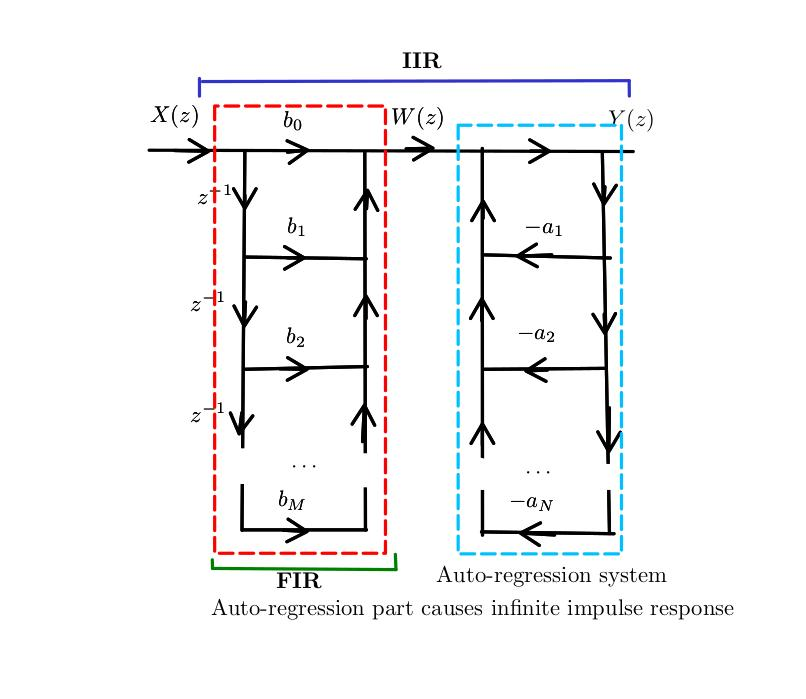
\includegraphics[width=0.7\textwidth]{7.jpg}
			\caption{Signal-flow graph of FIR and IIR system}			\label{fig:re7}

		\end{figure}
\end{frame}
\end{document}
